%%%%%%%%%%%%%%%%%%%%%%%%%%%%%%%%%%%%%%%%%%%%%%
%Lab report writeup based on template by Derek Hildreth
%%%%%%%%%%%%%%%%%%%%%%%%%%%%%%%%%%%%%%%%%%%%%%

%\documentclass[aps,letterpape,10pt]{revtex4}
\documentclass[aps,letterpaper,10pt]{article}
%\documentclass{article}

\usepackage{graphicx} % For images
\usepackage{float}    % For tables and other floats
\usepackage{verbatim} % For comments and other
\usepackage{amsmath}  % For math
\usepackage{amssymb}  % For more math
\usepackage{fullpage} % Set margins and place page numbers at bottom center
\usepackage{subfig}   % For subfigures
\usepackage[usenames,dvipsnames]{color} % For colors and names
\usepackage{fancyhdr} %headers
\usepackage{listings} %for code
\usepackage{color} %to color code
\usepackage{wrapfig} % for inline images

%Color and code setup
\definecolor{dkgreen}{rgb}{0,0.6,0}
\definecolor{gray}{rgb}{0.5,0.5,0.5}
\definecolor{mauve}{rgb}{0.58,0,0.82}
\definecolor{codebg}{rgb}{.95,.95,.98}

\lstset{ %
	language=Java,
	tabsize=4, 
	numbers=left,
	numberstyle=\footnotesize,
	backgroundcolor=\color{codebg},
	breaklines=true,
	breakatwhitespace=true,
	basicstyle=\small,
	numberstyle=\tiny\color{black},
	showstringspaces=false,
	keywordstyle=\color{blue}, 
	stringstyle=\color{dkgreen},
	commentstyle=\color{gray},
	frame=single,
	title = \texttt{\lstname}
	}

%%%%%%%%%%%%

%HEADER FORMATING%%%%%%%%%%%%%
\pagestyle{fancy}
\headheight 23pt
\setlength{\headsep}{20pt}
\lhead{PHYS 251 - Prof. Tom Witten \\ Project 3}
\rhead{A. Athanassiadis\\Due 11/9/2012}
%%%%%%%%%%%%%%%%%%%%%%%%

%Custom Definitions%%%%%%%%%%%%%%%
\newcommand{\ttt}{\texttt}
%%%%%%%%%%%%%%%%%%%%%%%%

\begin{document}

\section{Logistic Map}

To begin understand the scaling properties in period-doubling systems, I looked at the familiar iterative map defined by
$$ f_r (x) = r x (1-x). $$

As shown in \ttt{IterMap.java}, I used Newton's method to find out when $f^{(2^k)} _r (x_m) = x_m.$ Finding the $\tilde{r}_k$ that satisfy this condition for each $k$ yields a sequence that must converge to the same value, $r_\infty$, as the $r_k$ which are the bifurcation points of $f$. To understand how $r_k\rightarrow r_\infty$, the ratio $\delta$ can be calculated as a scaling parameter. A similar parameter $\alpha$ can also be calculated, which describes the scaling of $f\rightarrow f_{r_\infty}$ by tracking the parameter. The calculated results are shown in the following table:

\begin{center}
\begin{tabular}{|c|c|c|c|c|}
\hline
$k$&$r_{sk}$&$\delta$&$y$&$\alpha$\\
\hline
01&2.0000&--&0.5000&--\\
02&3.2361&--&0.8090&--\\
03&3.4986&4.7089&0.3836&0.7264\\
04&3.5546&4.6808&0.5460&2.6199\\
05&3.5667&4.6630&0.4817&2.5252\\
06&3.5692&4.6684&0.5073&2.5074\\
07&3.5698&4.6690&0.4971&2.5038\\
08&3.5699&4.6692&0.5012&2.5031\\
09&3.5699&4.6692&0.4995&2.5029\\
10&3.5699&4.6692&0.5002&2.5029\\
\hline
\end{tabular}
\end{center}


\section{Universality}
When the function is changed, there is no {\emph a priori} reason to assume that the behavior of $r$ and $f$ will be the same as the logistic map. Using the function $$G_r(x) = rx^2\sqrt{1-x}$$ I performed the same analysis of $\delta$ and $\alpha$. That these two numbers converge to the same values as for the iterative map should in fact not be surprising. The derivation of these scaling parameters revealed that for any function ``like'' the logistic map (single quadratic maximum, f(0) = 0) should scale like the logistic map. Thus choice of function became an irrelevant parameter. The table of $\delta$ and $\alpha$ are presented here, along with the bifurcation diagram for $G_r$. The code used to calculate these was \ttt{IterMap2.java}.

\begin{center}
\begin{tabular}{|c|c|c|}
\hline
$k$&$\delta$&$\alpha$\\
\hline
01&--&--\\
02&--&--\\
03&4.3977&0.6785\\
04&4.6123&2.2768\\
05&4.6578&2.6430\\
06&4.6668&2.4575\\
07&4.6687&2.5228\\
08&4.6691&2.4953\\
09&4.6692&2.5060\\
10&4.6696&2.5017\\
\hline
\end{tabular}
\begin{figure}[!h]
\centering
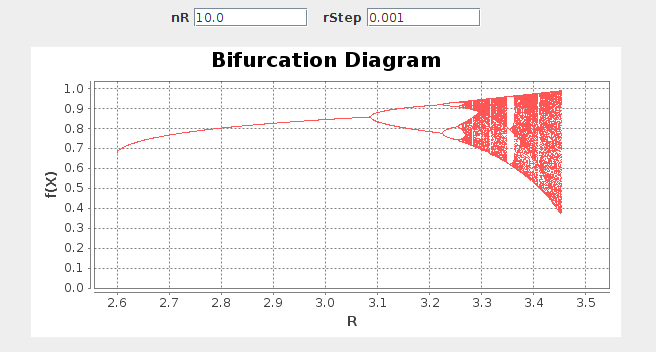
\includegraphics[width=.5\textwidth]{IterMap2.png}
\end{figure}
\end{center}


\section{Renormalization Groups}

The emergent universality in the scaling of iterated maps begs the question of how odd our function can be and still behave similarly. To check this, I used a function with a $3/2$ power cusp defined by $$f(x) = r\left( (\frac{1}{2})^{3/2} - |x-\frac{1}{2}|^\frac{1}{2}  \right).$$ Performing the same calculations as below yielded the table and bifurcation diagram below (see \ttt{IterMap3.java}):

\begin{centering}
\begin{figure}[!h]
\begin{tabular}{|c|c|c|}
\hline
$k$&$\delta$&$\alpha$\\
\hline
01&--&--\\
02&--&--\\
03&3.8261&0.7856\\
04&3.7812&3.6168\\
05&3.7918&3.4416\\
06&3.7982&3.4019\\
07&3.7999&3.3921\\
08&3.8004&3.3896\\
09&3.8005&3.3889\\
10&3.8005&3.3887\\
\hline
\end{tabular}
\end{figure}

\begin{figure}[!h]
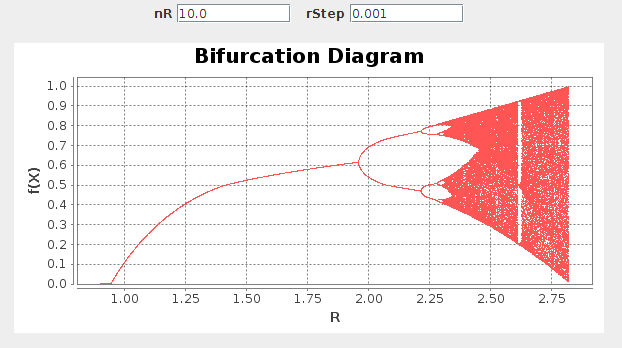
\includegraphics[width=.5\textwidth]{IterMap3.png}
\end{figure}
\end{center}

The surprising result here is that the power laws governing approach to $r_\infty$ are have different coefficients than for the logistic map! However, this may not be as crazy as it seems. The derivation of $g(r)$ is the same for all functions $f$ with a single maximum, however, there is an assumption that we used in the estimation of the scaling exponents which is no longer valid. In it, we approximated that $g(z)$ the limiting function of $f$ as $r\rightarrow r_\infty$ could be approximated as 
$$g(z)\approx A + Bz^2$$ 
near $z=0$ because of the quadratic maximum. However, this expansion is not the right expansion for $g$ when $f$ is the cusped function above. In this case, we must approximate $$g(x)\approx A + B|z|^{3/2}.$$

All other assumptions that led to the Feigenbaum equation were valid, and thus we can use this minor adjustment to reevaluate our expectations for $\alpha$ in this new system.

Feigenbaum can take the form $$g(z) = -\alpha g(g(-z/\alpha)).$$ With this equation and the approximation, we can write:

\begin{eqnarray*}
g(z) & = & A - B|z|^{3/2} \\
g(g(z)) & = & A - B|A - B|z|^{3/2}|^{3/2}\\
 & = & A - BA^{3/2}|1-\frac{B}{A}|z|^{3/2}|^{3/2}
\end{eqnarray*}

At this point, we can exploit the fact that $z$ is small, and expand the term inside the absolute values as $(1+\epsilon)^{3/2} \approx 1 + \frac{3}{2}\epsilon.$ Doing this and substituting into the Feigenbaum eq. we find that

$$ A - B|z|^{3/2} = -\alpha A + \alpha B A^{3/2} (1 - \frac{3B}{2A\alpha^{3/2}} |z|^{3/2}) $$

Equating the coefficients of like terms, we find that 
\begin{eqnarray*}
A & = & -\alpha A + \alpha B A^{3/2} \\
\Rightarrow BA^{1/2} & = & \frac{1 + \alpha}{\alpha} \\
B & = & \frac{3B^2A^{1/2}}{2\alpha^{1/2}} \\
\Rightarrow 2\alpha^{1/2} & = & 3 \frac{1 + \alpha}{\alpha} \\
\therefore \hspace{2em} 0 & = & 9 (1 + \alpha)^2 - 4\alpha^3
\end{eqnarray*}

Using the previously discovered value of $\alpha$ and \ttt{NSolve.java}, I numerically solved for the root of this final equation and calculated an estimate of 
$$\alpha \approx 3.65.$$

Comparing this to the value attained by iteration, we find a discrepancy of less than $10\%$.
To improve the agreement, the approximate Feigenbaum equation could include higher order terms.

Regardless of numerical precision, the existence of a second scaling behavior supports the existence of Universality classes, which can broadly describe the behavior of certain functions that meet requirements specific to the class. Here we have seen a new universality class of functions with $3/2$ power law cusps. While the period doubling and convergence to $r_\infty$ behavior are the same as for functions with quadratic maxima, the manner in which they converge differs significantly.

\newpage
\section{Code}
\lstinputlisting{../IterMap.java}
\newpage
\lstinputlisting{../IterMap2.java}
\newpage
\lstinputlisting{../IterMap3.java}
\newpage
\lstinputlisting{../NSolve.java}

\end{document} 
